\section{Model\-ND  Class Reference}
\label{classModelND}\index{ModelND@{Model\-ND}}
Simple axis-parallel motions in an N-dimensional space. 


{\tt \#include $<$modelmisc.h$>$}

Inheritance diagram for Model\-ND::\begin{figure}[H]
\begin{center}
\leavevmode
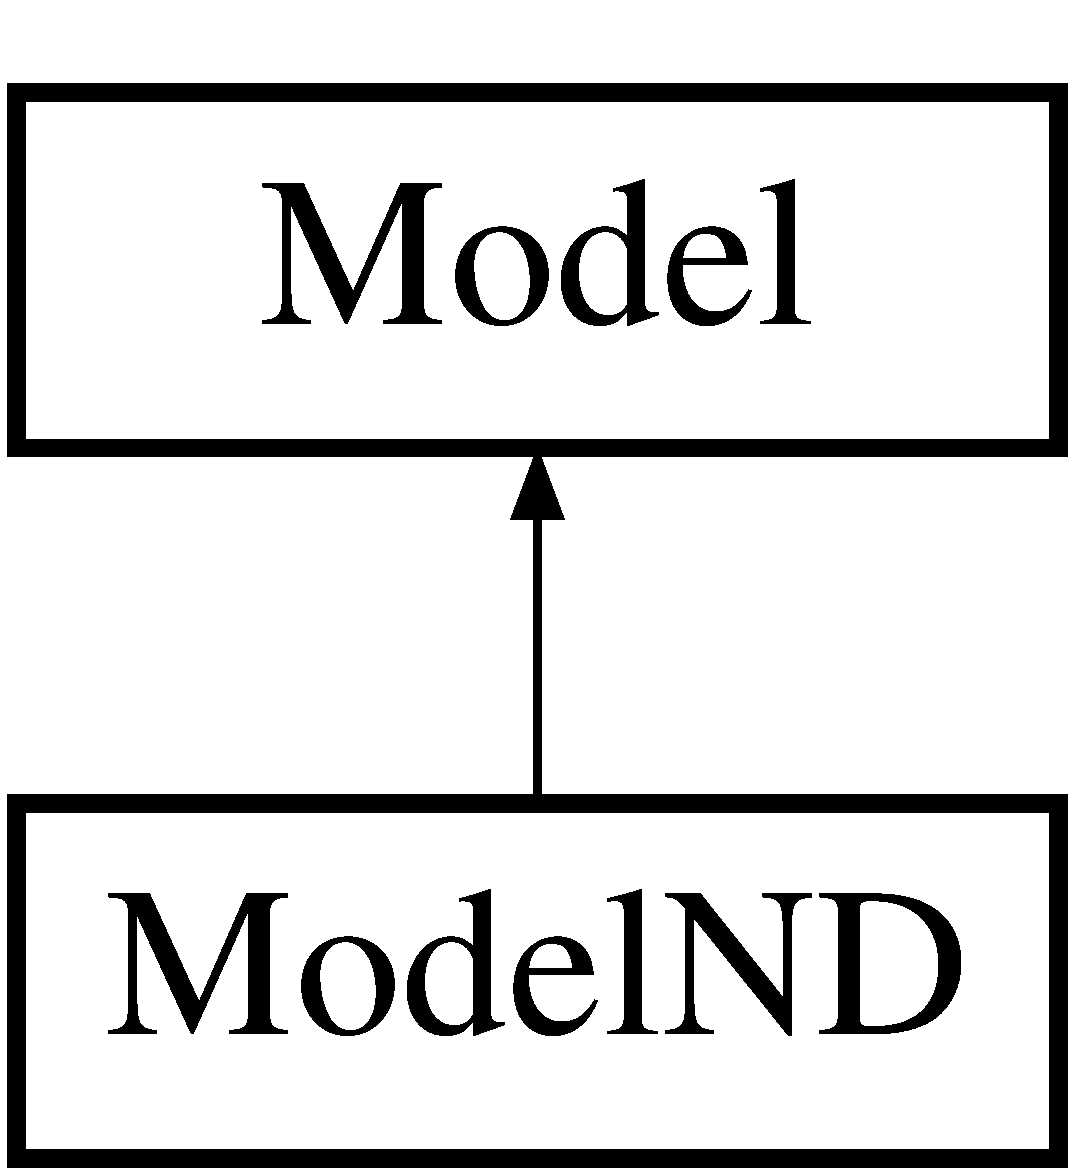
\includegraphics[height=2cm]{classModelND}
\end{center}
\end{figure}
\subsection*{Public Methods}
\begin{CompactItemize}
\item 
{\bf Model\-ND} (string path)
\item 
virtual {\bf $\sim$Model\-ND} ()
\item 
virtual {\bf MSLVector} {\bf State\-To\-Configuration} (const {\bf MSLVector} \&x)
\begin{CompactList}\small\item\em A method that converts a {\bf Model} {\rm (p.\,\pageref{classModel})} state in to a {\bf Geom} {\rm (p.\,\pageref{classGeom})} configuration.\item\end{CompactList}\item 
virtual {\bf MSLVector} {\bf Integrate} (const {\bf MSLVector} \&x, const {\bf MSLVector} \&u, const double \&h)
\begin{CompactList}\small\item\em Perform integration from state x, using input u, over time step h.\item\end{CompactList}\item 
virtual {\bf MSLVector} {\bf State\-Transition\-Equation} (const {\bf MSLVector} \&x, const {\bf MSLVector} \&u)
\begin{CompactList}\small\item\em The state transition equation, or equations of motion, xdot=f(x,u).\item\end{CompactList}\end{CompactItemize}
\subsection*{Public Attributes}
\begin{CompactItemize}
\item 
double {\bf Corridor\-Width}
\end{CompactItemize}


\subsection{Detailed Description}
Simple axis-parallel motions in an N-dimensional space.



\subsection{Constructor \& Destructor Documentation}
\index{ModelND@{Model\-ND}!ModelND@{ModelND}}
\index{ModelND@{ModelND}!ModelND@{Model\-ND}}
\subsubsection{\setlength{\rightskip}{0pt plus 5cm}Model\-ND::Model\-ND (string {\em path} = \char`\"{}\char`\"{})}\label{classModelND_a0}


\index{ModelND@{Model\-ND}!~ModelND@{$\sim$ModelND}}
\index{~ModelND@{$\sim$ModelND}!ModelND@{Model\-ND}}
\subsubsection{\setlength{\rightskip}{0pt plus 5cm}Model\-ND::$\sim$Model\-ND ()\hspace{0.3cm}{\tt  [inline, virtual]}}\label{classModelND_a1}




\subsection{Member Function Documentation}
\index{ModelND@{Model\-ND}!Integrate@{Integrate}}
\index{Integrate@{Integrate}!ModelND@{Model\-ND}}
\subsubsection{\setlength{\rightskip}{0pt plus 5cm}{\bf MSLVector} Model\-ND::Integrate (const {\bf MSLVector} \& {\em x}, const {\bf MSLVector} \& {\em u}, const double \& {\em h})\hspace{0.3cm}{\tt  [virtual]}}\label{classModelND_a3}


Perform integration from state x, using input u, over time step h.



Reimplemented from {\bf Model} {\rm (p.\,\pageref{classModel_a5})}.\index{ModelND@{Model\-ND}!StateToConfiguration@{StateToConfiguration}}
\index{StateToConfiguration@{StateToConfiguration}!ModelND@{Model\-ND}}
\subsubsection{\setlength{\rightskip}{0pt plus 5cm}{\bf MSLVector} Model\-ND::State\-To\-Configuration (const {\bf MSLVector} \& {\em x})\hspace{0.3cm}{\tt  [virtual]}}\label{classModelND_a2}


A method that converts a {\bf Model} {\rm (p.\,\pageref{classModel})} state in to a {\bf Geom} {\rm (p.\,\pageref{classGeom})} configuration.



Reimplemented from {\bf Model} {\rm (p.\,\pageref{classModel_a8})}.\index{ModelND@{Model\-ND}!StateTransitionEquation@{StateTransitionEquation}}
\index{StateTransitionEquation@{StateTransitionEquation}!ModelND@{Model\-ND}}
\subsubsection{\setlength{\rightskip}{0pt plus 5cm}{\bf MSLVector} Model\-ND::State\-Transition\-Equation (const {\bf MSLVector} \& {\em x}, const {\bf MSLVector} \& {\em u})\hspace{0.3cm}{\tt  [virtual]}}\label{classModelND_a4}


The state transition equation, or equations of motion, xdot=f(x,u).



Reimplemented from {\bf Model} {\rm (p.\,\pageref{classModel_a3})}.

\subsection{Member Data Documentation}
\index{ModelND@{Model\-ND}!CorridorWidth@{CorridorWidth}}
\index{CorridorWidth@{CorridorWidth}!ModelND@{Model\-ND}}
\subsubsection{\setlength{\rightskip}{0pt plus 5cm}double Model\-ND::Corridor\-Width}\label{classModelND_m0}




The documentation for this class was generated from the following files:\begin{CompactItemize}
\item 
{\bf modelmisc.h}\item 
{\bf modelmisc.C}\end{CompactItemize}
